\documentclass[11pt]{beamer}
\beamertemplatenavigationsymbolsempty
\usetheme{Penn} 

\logo{}
\newcommand{\TODO}[1]{{\color{red}#1}}

\usepackage{epsfig, amsfonts, amsbsy, amsmath}
\usepackage{color}
\usepackage{amsmath}
\usepackage{amssymb}
\usepackage{scrextend}
\usepackage{float}
\usepackage{color}
\usepackage{graphicx} 
\usepackage{xspace} 
\usepackage{caption}
\usepackage{subcaption}
\usepackage{url}
\usepackage{natbib}
\usepackage[T1]{fontenc}
\usepackage[utf8]{inputenc}
\usepackage{multirow}

% Copyright 2007 by Till Tantau
%
% This file may be distributed and/or modified
%
% 1. under the LaTeX Project Public License and/or
% 2. under the GNU Public License.
%
% See the file doc/licenses/LICENSE for more details.

\ProvidesPackageRCS $Header: /cvsroot/latex-beamer/latex-beamer/themes/color/beamercolorthemepenn.sty,v 1.4 2007/01/28 20:48:24 tantau Exp $

\definecolor{pennred}{cmyk}{0.75, 0.4, 1, 0.4}
\definecolor{pennblue}{cmyk}{1,0.7,0,0.30}



\mode<presentation>

\setbeamercolor*{palette primary}{use=structure,fg=white,bg= pennblue}
\setbeamercolor*{palette secondary}{use=structure,fg=white,bg= pennblue}
\setbeamercolor*{palette tertiary}{use=structure,fg=white,bg= pennblue}
\setbeamercolor*{palette quaternary}{fg=white,bg= pennblue}

\setbeamercolor*{sidebar}{use=structure,bg= pennblue}
  
\setbeamercolor*{palette sidebar primary}{use=structure,fg=structure.fg!10}
\setbeamercolor*{palette sidebar secondary}{fg=white}
\setbeamercolor*{palette sidebar tertiary}{use=structure,fg=structure.fg!50}
\setbeamercolor*{palette sidebar quaternary}{fg=white}

\setbeamercolor*{titlelike}{parent=palette primary}

\setbeamercolor*{separation line}{}
\setbeamercolor*{fine separation line}{}

\setbeamercolor{itemize item}{fg=pennblue}
\setbeamercolor{itemize subitem}{fg=pennblue}
\setbeamercolor{itemize subsubitem}{fg=pennblue}
\setbeamercolor{enumerate item}{fg=pennblue}
\setbeamercolor{enumerate subitem}{fg=pennblue}
\setbeamercolor{enumerate subsubitem}{fg=pennblue}
\setbeamercolor{description item}{fg=pennblue}


\mode
<all>

 \setbeamercovered{invisible}
 

\begin{document}

\author[]{\begin{tabular}{c} 
\\ \textbf{Team:} \\
{\small Martin Blapp}\\
{\small Doruk Çetin}\\
{\small Bernhard Kratzwald}\\
%{\small ... (order names alphabetically)}
\end{tabular}}

\date{Spring 2019}

\title{Combining Human and Machine Decisions}


\frame{
\begin{center}
{\small Fairness, Explainability, and Accountability for ML}
\end{center}
\titlepage}

\begin{frame}{Why combine human and machine decisions?}
\begin{itemize}
	\setlength\itemsep{1em}
	\item Decision problems that need human involvement
	\begin{itemize}
	\item jail-or-release
	\item stop-and-frisk
	\item accept-or-reject (e.g., academics, credits, etc.	
	\end{itemize}
	\item Human decision makers can profit from Machine decisions
		\begin{itemize}
		\item reduce the workload
		\item increase accuracy
	\end{itemize}
\end{itemize}
\end{frame}

\begin{frame}{Human and machine decisions}
\begin{itemize}
	\item How do we combine human and machine decisions?
	\item How are humans influenced by machine predictions? 
\end{itemize}
\centering
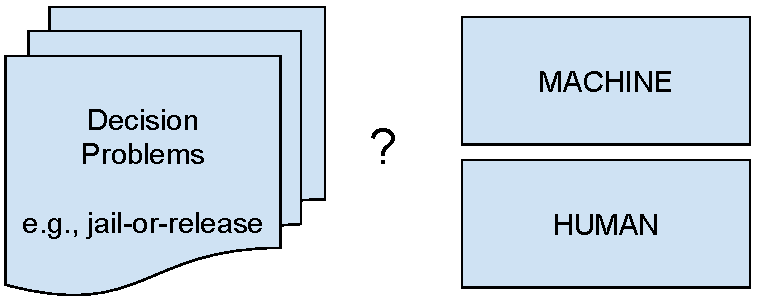
\includegraphics[width=0.5\textwidth]{Figures/problem_statement.pdf}

\end{frame}

\begin{frame}{Default Pattern}
\begin{itemize}
\setlength\itemsep{5pt}%

\item + Human remains the upper hand and makes the final decision
\item + Clear responsibility

\item -- What about fairness?
\item -- How is the human influenced by the machine prediction?
\item \TODO{change title add reference}
\end{itemize}

\begin{figure}[t!]
    \centering
        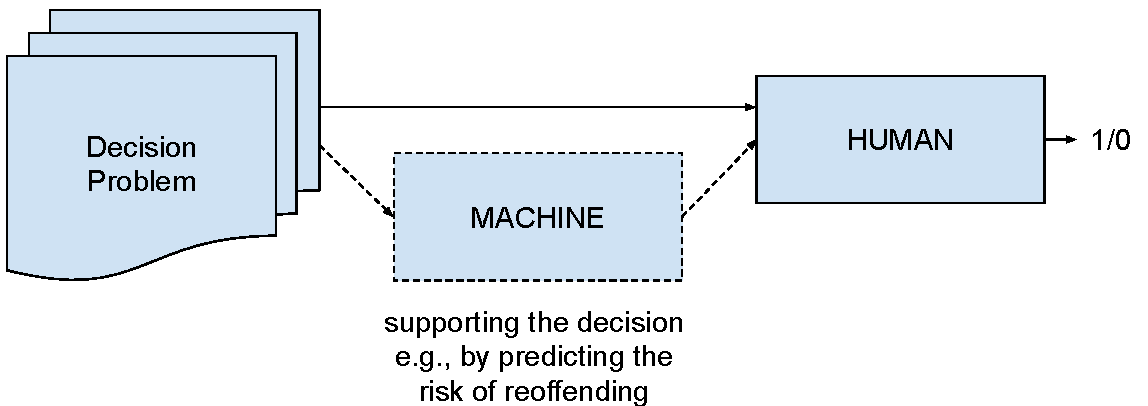
\includegraphics[width=0.8\textwidth]{Figures/human_decision.pdf}
\end{figure}
\end{frame}


\begin{frame}{Paper 3}
\end{frame}

\begin{frame}{Paper 3}
\end{frame}


\begin{frame}{Paper 3}
\end{frame}


\begin{frame}{Paper 3}
\end{frame}


\begin{frame}{Alternative pattern: Learn to defect}

\begin{figure}[t!]
	\centering
	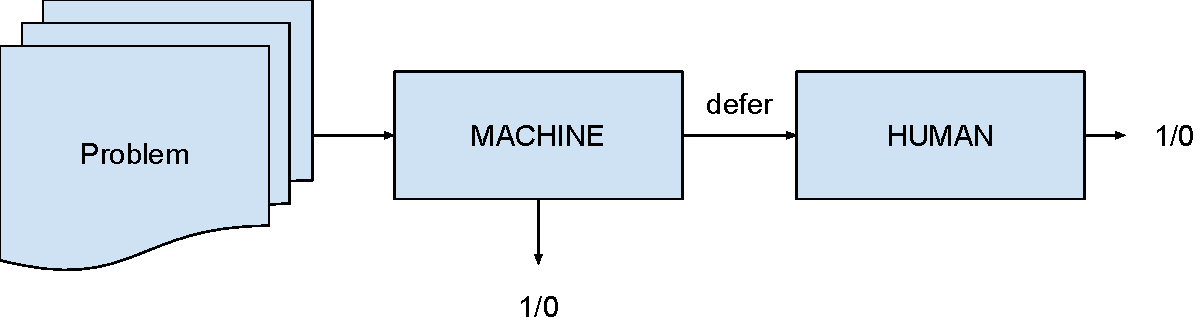
\includegraphics[width=0.8\textwidth]{Figures/defect.pdf}
\end{figure}
\end{frame}

\begin{frame}{Paper 1}
\end{frame}

\begin{frame}{Paper 1}
\end{frame}


\begin{frame}{Paper 1}
\end{frame}


\begin{frame}{Paper 1}
\end{frame}


\begin{frame}{Alternative pattern: Problem matching}
	\centering
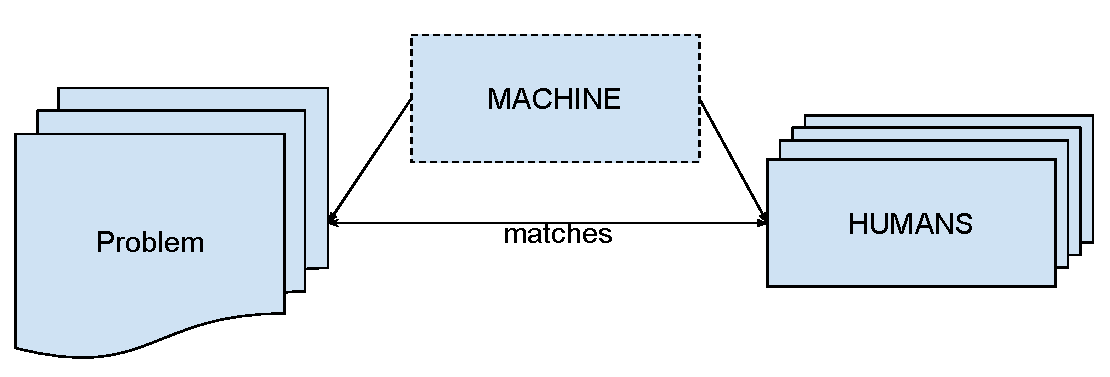
\includegraphics[width=0.8\textwidth]{Figures/matching.pdf}
\end{frame}


\begin{frame}{Paper 2}
\end{frame}

\begin{frame}{Paper 2}
\end{frame}


\begin{frame}{Paper 2}
\end{frame}


\begin{frame}{Paper 2}
\end{frame}

\begin{frame}{Conclusion}
\begin{table}[]
	\begin{tabular}{cl}
		\multirow{3}{*}{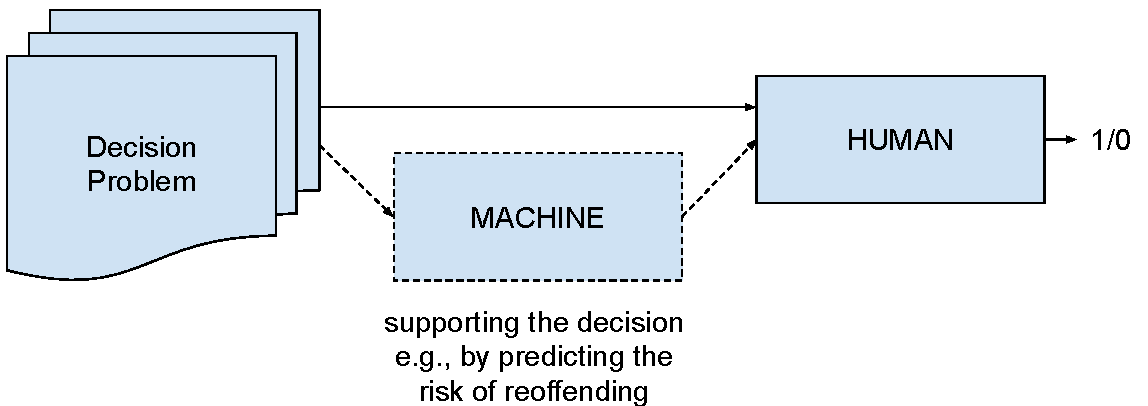
\includegraphics[width=0.4\textwidth]{Figures/human_decision.pdf}}&   + Benefit 1 		 \\
		& + Benefit 2\\
		& -- Disadvantage 1\\ 
		&\\
		\hline
		&\\
		\multirow{3}{*}{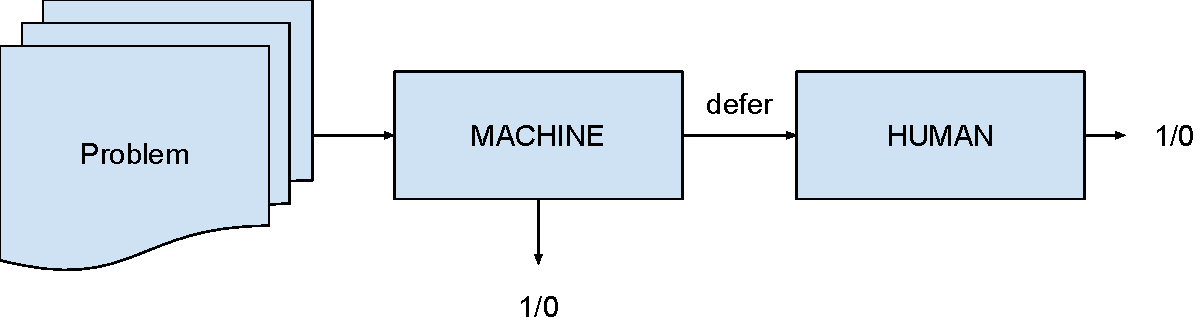
\includegraphics[width=0.4\textwidth]{Figures/defect.pdf}}&   	+ Text			\\
		& -- Lorem \\
		& -- Ipso \\
		&\\
		\hline
		&\\
		\multirow{3}{*}{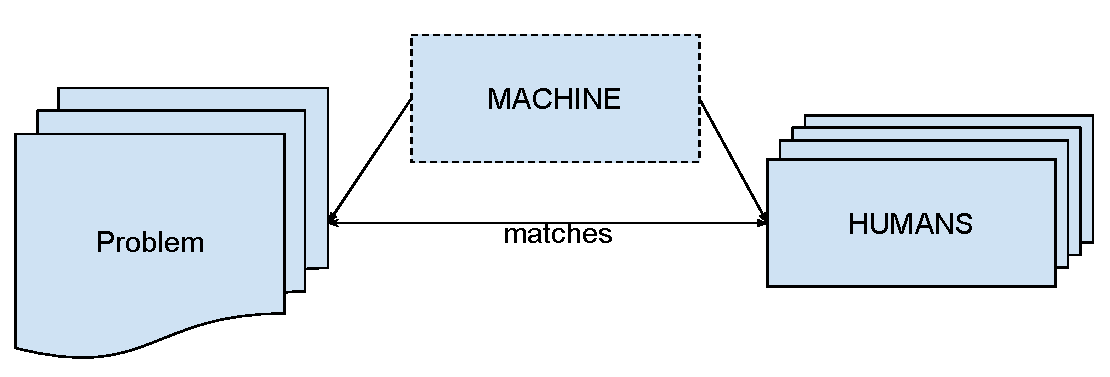
\includegraphics[width=0.4\textwidth]{Figures/matching.pdf}}&   + Dolor				\\
		& + More \\
		& -- Text \\
	\end{tabular}
\end{table}
\end{frame}

\begin{frame}{Other patterns worth mentioning}
\end{frame}

\begin{frame}{References}
\end{frame}

\end{document}
